% Minh họa một trang: ý tưởng + kết quả (25/10/2026). Biên dịch: xelatex minh_hoa.tex
% Ảnh: khung hình cắt từ video đánh giá outputs/videos/2026-10-25/A_vs_D_finetuned/ (C1 seed 400000, C4 seed 400003).
% Mốc thời gian trên trục: sự kiện ghi trong tập đánh giá C1 seed 400000 (A_ft, D_ft).
\documentclass[10pt]{article}
\usepackage[a4paper, margin=1.1cm]{geometry}
\usepackage{fontspec}
\usepackage[english, main=vietnamese]{babel}
\IfFontExistsTF{Times New Roman}
  {\setmainfont{Times New Roman}}
  {\setmainfont{texgyretermes}[Extension=.otf, UprightFont=*-regular,
     BoldFont=*-bold, ItalicFont=*-italic, BoldItalicFont=*-bolditalic]}
\usepackage{graphicx, array}
\graphicspath{{fig/}}
\usepackage{xcolor}
\usepackage{tikz}
\usetikzlibrary{positioning, arrows.meta}
\usepackage{pgfplots}
\pgfplotsset{compat=1.18}
\setlength{\parindent}{0pt}
\setlength{\parskip}{2pt}
\pagestyle{empty}
\definecolor{colA}{RGB}{140,140,140}
\definecolor{colD}{RGB}{31,119,180}
\definecolor{colW}{RGB}{214,39,40}
\newcommand{\phan}[1]{\par\smallskip{\large\bfseries #1}\par}
\newcommand{\so}[1]{\tikz[baseline=(n.base)]\node[circle, fill=black, text=white, inner sep=1pt, font=\scriptsize\bfseries](n){#1};}
\newcommand{\anh}[1]{\includegraphics[width=4.75cm]{#1}}

\begin{document}

\begin{center}
{\large\bfseries Học chính sách hành động cộng tác người - robot có nhận thức ý định}\\[1pt]
Minh họa ý tưởng và kết quả, 25/10/2026
\end{center}
\vspace{-6pt}

\phan{Ý tưởng}
Người đang làm việc, lát nữa sẽ cần robot đưa cho một lon (đỏ). Robot nên đưa \textbf{lúc nào}?
\begin{itemize}\setlength{\itemsep}{0pt}
  \item \textcolor{colA}{\textbf{A (cách thường):}} chờ người đưa tay ra xin rồi mới đi lấy lon $\Rightarrow$ người phải đứng chờ.
  \item \textcolor{colD}{\textbf{D (đề xuất):}} dự báo chuyển động tay người 1\,s tới, robot lấy lon sẵn và tới tay người đúng lúc;
  nếu đoán sai hoặc người đổi ý thì robot dừng lại và sửa. A và D cùng là ACT, cùng số bước train; A không có nhánh dự báo.
\end{itemize}
\begin{center}
\vspace{-4pt}
\begin{tikzpicture}[font=\footnotesize, >={Stealth[length=4pt]}, node distance=2mm and 6mm,
  box/.style={draw, rounded corners=2pt, align=center, inner sep=2pt, minimum height=6mm}]
  \node[box] (kp) {tay người 0.4\,s vừa qua};
  \node[box, fill=gray!15, right=of kp] (mc) {ManiCast};
  \node[box, right=of mc] (fc) {dự báo tay người 1\,s tới};
  \node[box, fill=colD!15, right=of fc, minimum height=13mm] (act) {ACT\\(chính sách robot)};
  \node[box, below=of fc] (cam) {3 camera + trạng thái robot};
  \node[box, right=of act] (out) {hành động robot};
  \draw[->] (kp) -- (mc); \draw[->] (mc) -- (fc); \draw[->] (fc) -- (act.west |- fc);
  \draw[->] (cam) -- (act.west |- cam);
  \draw[->] (act) -- (out);
\end{tikzpicture}
\end{center}
\vspace{-6pt}

\phan{1. Cùng một tình huống, cùng thời điểm (dự báo đúng, C1)}
\begin{center}
\vspace{-4pt}
\setlength{\tabcolsep}{2pt}
\begin{tabular}{@{}m{2.2cm}ccc@{}}
 & \so{1}\ $t=4.0$\,s: người còn làm việc & \so{2}\ $t=8.0$\,s: người vừa đưa tay xin & \so{3}\ $t=9.6$\,s \\[1pt]
\textcolor{colA}{\textbf{A}}\newline\scriptsize chờ cử chỉ & \anh{c1_A_t40} & \anh{c1_A_t80} & \anh{c1_A_t96} \\
 & \scriptsize robot đứng chờ & \scriptsize robot vẫn chờ & \scriptsize robot mới đi lấy lon \\[1pt]
\textcolor{colD}{\textbf{D}}\newline\scriptsize dự báo ý định & \anh{c1_D_t40} & \anh{c1_D_t80} & \anh{c1_D_t96} \\
 & \scriptsize robot đã cầm lon sẵn & \scriptsize robot đã ở gần tay người & \scriptsize robot đang trao lon \\
\end{tabular}
\end{center}
\vspace{-8pt}

% Trục thời gian của chính tập trên (giây): người xong việc 7.1, tay sẵn sàng nhận 7.95;
% A cầm lon 11.35, tới tay 14.5, trao xong 16.15; D cầm lon 2.75, tới tay 9.4, trao xong 11.05.
\begin{center}
\begin{tikzpicture}[x=0.9cm, y=0.6cm, font=\footnotesize]
  \foreach \t in {0,2,...,16} { \draw[gray!40] (\t,-0.4) -- (\t,2.4); \node[below, gray] at (\t,-0.4) {\t\,s}; }
  % người
  \node[left] at (-0.1,2) {\textbf{Người}};
  \fill[gray!25] (0,1.8) rectangle (7.1,2.2); \node at (3.55,2) {đang làm việc};
  \fill[orange!70] (7.1,1.8) rectangle (7.95,2.2); \node[above, font=\scriptsize] at (7.2,2.2) {đưa tay xin};
  % A
  \node[left] at (-0.1,1) {\textcolor{colA}{\textbf{A}}};
  \fill[colW!25] (7.95,0.8) rectangle (14.5,1.2); \node[colW!80!black, font=\scriptsize] at (12.95,1) {người chờ 6.6\,s};
  \fill[colA] (11.35,1) circle (3pt); \node[above, font=\scriptsize] at (11.35,1.15) {cầm lon};
  \draw[colA, very thick] (14.5,0.75) -- (14.5,1.25); \node[left, font=\scriptsize] at (14.45,0.55) {tới tay};
  \draw[colA, very thick] (16.15,0.75) -- (16.15,1.25);
  \node[colA, font=\scriptsize\bfseries, right] at (16.15,1) {xong 16.2\,s};
  % D
  \node[left] at (-0.1,0) {\textcolor{colD}{\textbf{D}}};
  \fill[colW!25] (7.95,-0.2) rectangle (9.4,0.2); \node[colW!80!black, font=\scriptsize, left] at (7.9,0) {người chờ 1.5\,s};
  \fill[colD] (2.75,0) circle (3pt); \node[right, font=\scriptsize] at (2.85,0) {cầm lon};
  \draw[colD, very thick] (9.4,-0.25) -- (9.4,0.25); \node[right, font=\scriptsize] at (9.7,0) {tới tay};
  \draw[colD, very thick] (11.05,-0.25) -- (11.05,0.25);
  \node[colD, font=\scriptsize\bfseries, right] at (11.05,0) {xong 11.1\,s};
  % thời điểm của 3 ảnh
  \foreach \t/\k in {4.0/1, 8.0/2, 9.6/3} { \draw[dashed] (\t,-0.4) -- (\t,2.55); \node[circle, fill=black, text=white, inner sep=1pt, font=\scriptsize\bfseries] at (\t,2.75) {\k}; }
\end{tikzpicture}
\end{center}
\vspace{-6pt}

\phan{2. Khi người đổi ý (C4): D tự sửa}
\begin{center}
\vspace{-4pt}
\setlength{\tabcolsep}{2pt}
\begin{tabular}{@{}ccc@{}}
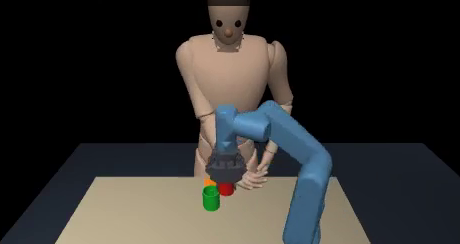
\includegraphics[width=4.3cm]{c4_D_t50} & 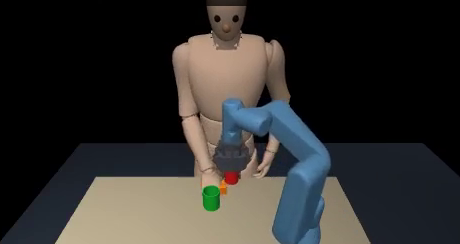
\includegraphics[width=4.3cm]{c4_D_t66} & 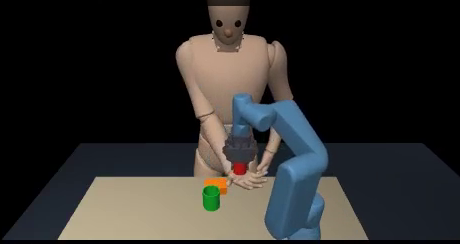
\includegraphics[width=4.3cm]{c4_D_t96} \\
\scriptsize $t=5.0$\,s: robot mang lon tới tay & \scriptsize $t=6.6$\,s: người rút tay $\Rightarrow$ robot dừng, giữ lon chờ & \scriptsize $t=9.6$\,s: người xin lại $\Rightarrow$ robot trao \\
\end{tabular}
\end{center}
\vspace{-6pt}
{\small Tương tự khi dự báo sai (C3: người với tay lấy cốc xanh của mình, trông giống xin): D không đưa nhầm, vẫn hoàn thành.}

\phan{3. Kết quả trên 120 tập test (30 tập mỗi trường hợp)}
{\small C1 dự báo đúng \;·\; C2 ý định mơ hồ \;·\; C3 dự báo sai \;·\; C4 người đổi ý \;·\; TB: trung bình 4 trường hợp}\\
{\small \textcolor{colA}{\rule{8pt}{8pt}} A (chờ cử chỉ) \quad \textcolor{colD}{\rule{8pt}{8pt}} D (dự báo ý định)}

\pgfplotsset{
  bar/.style={ybar, width=6.6cm, height=3.9cm, bar width=7pt, ymin=0, enlarge x limits=0.13,
    symbolic x coords={C1,C2,C3,C4,TB}, xtick=data, ytick style={draw=none}, xtick style={draw=none},
    axis x line*=bottom, axis y line*=left, ymajorgrids, grid style={gray!20},
    nodes near coords, nodes near coords style={font=\tiny, /pgf/number format/.cd, fixed, fixed zerofill, precision=1},
    tick label style={font=\footnotesize}, title style={font=\small\bfseries, yshift=-5pt}}}
\begin{tikzpicture}
\begin{axis}[bar, ymax=26, title={Thời gian hoàn thành [s] $\downarrow$}]
  \addplot[fill=colA, draw=none] coordinates {(C1,13.75) (C2,14.94) (C3,21.29) (C4,15.27) (TB,16.31)};
  \addplot[fill=colD, draw=none] coordinates {(C1,9.57) (C2,11.64) (C3,17.50) (C4,12.44) (TB,12.88)};
\end{axis}
\end{tikzpicture}\hfill
\begin{tikzpicture}
\begin{axis}[bar, ymax=9.5, title={Người phải chờ robot [s] $\downarrow$}]
  \addplot[fill=colA, draw=none] coordinates {(C1,6.04) (C2,5.84) (C3,5.46) (C4,7.55) (TB,6.22)};
  \addplot[fill=colD, draw=none] coordinates {(C1,1.81) (C2,2.61) (C3,1.64) (C4,5.36) (TB,2.88)};
\end{axis}
\end{tikzpicture}\hfill
\begin{minipage}[b]{5.0cm}
\small
\setlength{\tabcolsep}{3pt}
\textbf{Tỷ lệ thành công}\\[2pt]
\begin{tabular}{lcccc}
 & C1 & C2 & C3 & C4 \\ \hline
\textcolor{colA}{\textbf{A}} & 30/30 & 30/30 & 30/30 & 30/30 \\
\textcolor{colD}{\textbf{D}} & 28/30 & 26/30 & 30/30 & 30/30 \\
\end{tabular}\\[6pt]
\textbf{D so với A:}\\
$\bullet$ xong nhanh hơn \textbf{3.4\,s (21\,\%)}\\
$\bullet$ người chờ \textbf{6.2\,s $\to$ 2.9\,s}\\
$\bullet$ thành công 95\,\% (A 100\,\%)\\
$\bullet$ \textbf{0 va chạm} ở cả hai\\[4pt]
\end{minipage}

\vfill
{\footnotesize Mô phỏng MuJoCo, robot UR3e, người theo kịch bản. Kết quả trong mô phỏng còn khả quan hơn thực tế
(tập test gần tập train, tư thế người lấy chính xác từ mô phỏng).}

\end{document}
